\documentclass{beamer}
%\beamerdefaultoverlayspecification{<+->}

\usetheme{metropolis}
\usepackage{graphicx}
\usepackage{amsmath}
\usepackage{mathtools}
\usepackage{minted}

\title{Neural Networks for Image Classification}
\date{\today}
\author{Catalina Vajiac}
\institute{Saint Mary's College} 
\setminted{fontsize=\small, baselinestretch=1}
\begin{document}
  \maketitle

  \section{Introduction}
  \begin{frame}{Overview}
    \begin{itemize}
      \item Motivation for neural networks
      \item What is a neural network?
      \item Types of Neural Networks
      \begin{itemize}
        \item fully-connected
        \item deep
        \item convolutional
      \end{itemize}
      \item Gradient Descent
      \begin{itemize}
        \item Softmax classifier
        \item single-layer neural network
        \item arbitrary-layer neural network
      \end{itemize}
      \item Demonstration
        \begin{itemize}
          \item what is OOP?
          \item comparison of networks on MNIST
        \end{itemize}
    \end{itemize}
  \end{frame}

    \section{Image Classification}
  \begin{frame}{Goal: Image Classification}
     What is in this image?\\
    \begin{center}
      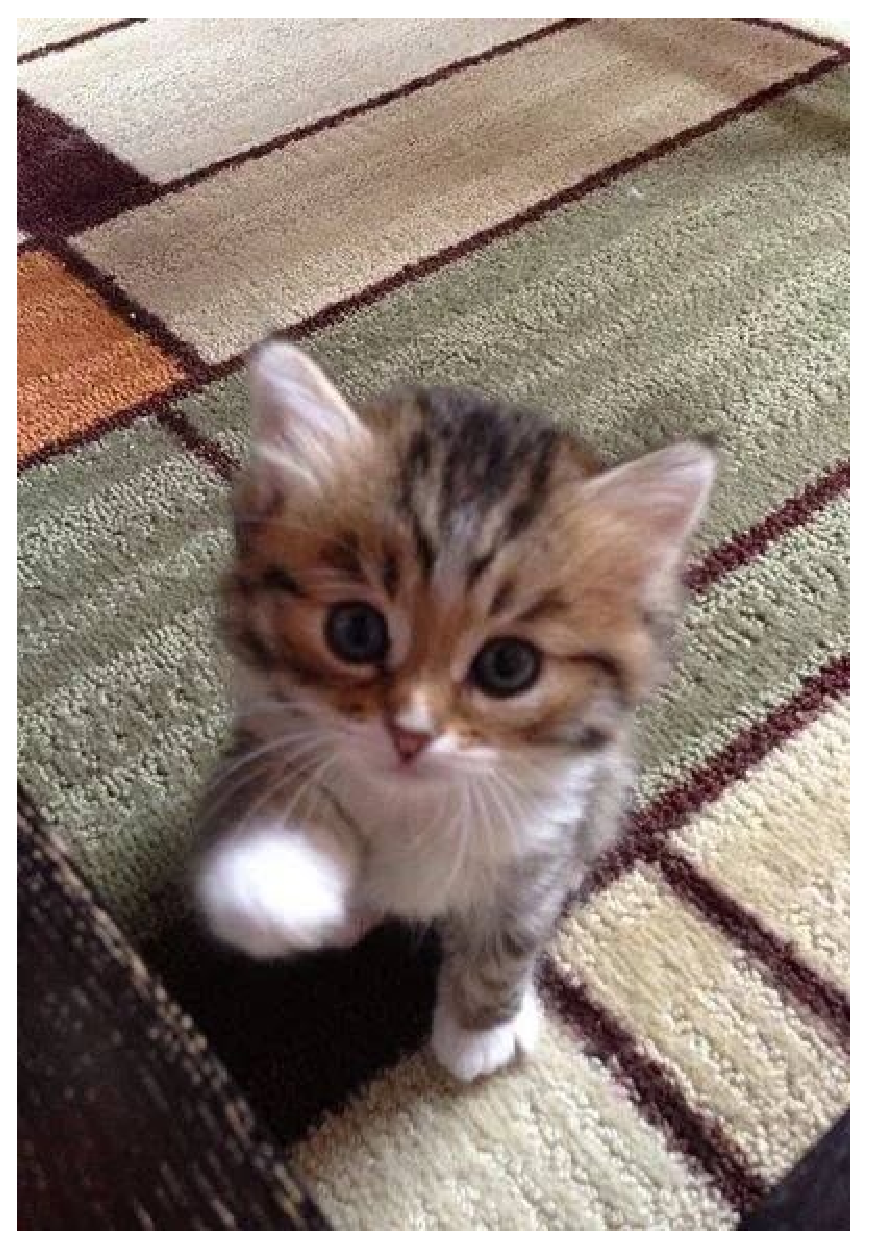
\includegraphics[width=1.5in]{../figures/kitty.eps}
    \end{center}
  \end{frame}

  \begin{frame}{Problem: Scale Variation}
    \begin{center}
      \includegraphics[width=3in]{../figures/kitty_scale_variation.eps}
    \end{center}
  \end{frame}

  \begin{frame}{Problem: Occlusion}
    \begin{center}
      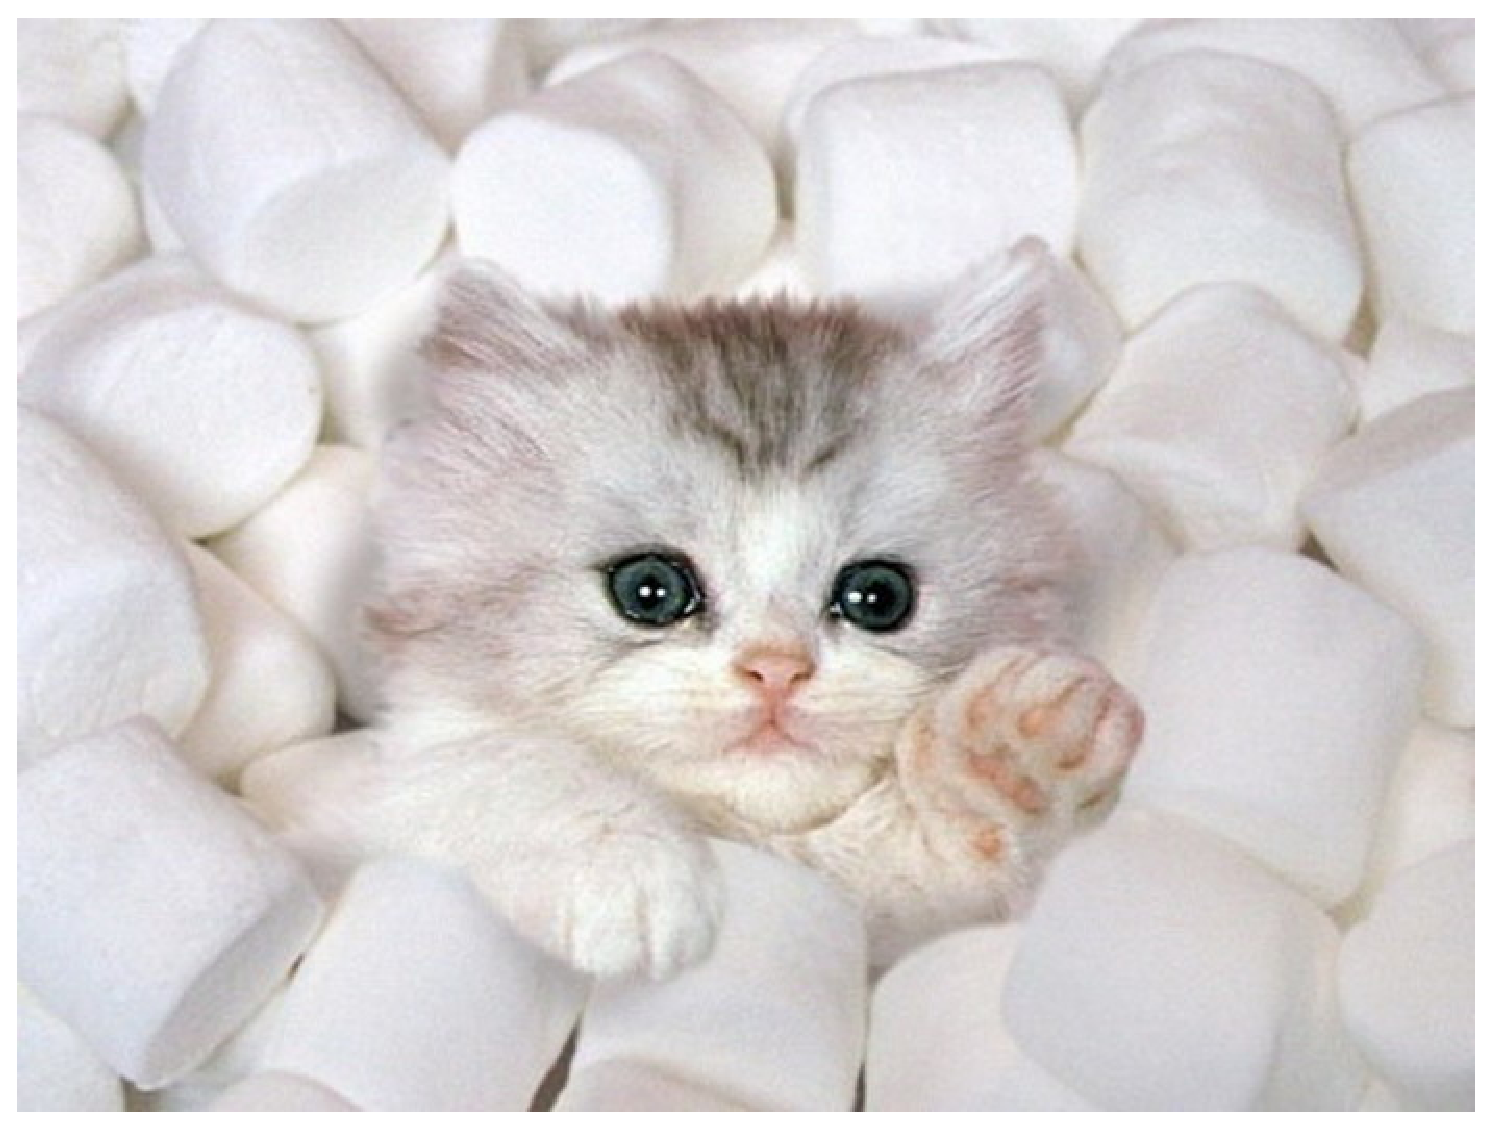
\includegraphics[width=3in]{../figures/kitty_occlusion.eps}
    \end{center}
  \end{frame}

  \begin{frame}{Problem: Deformation}
    \begin{center}
      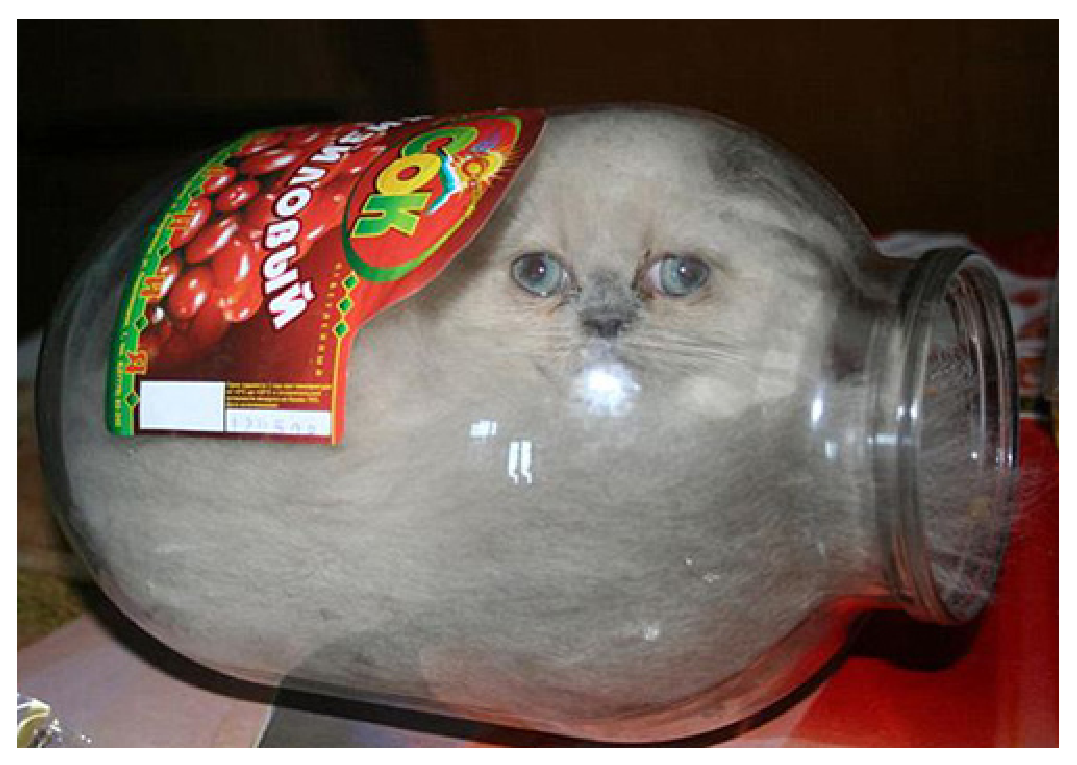
\includegraphics[width=3in]{../figures/cat_deformed.eps}
    \end{center}
  \end{frame}

  \begin{frame}{Problem: Intra-Class Variation}
    \begin{center}
      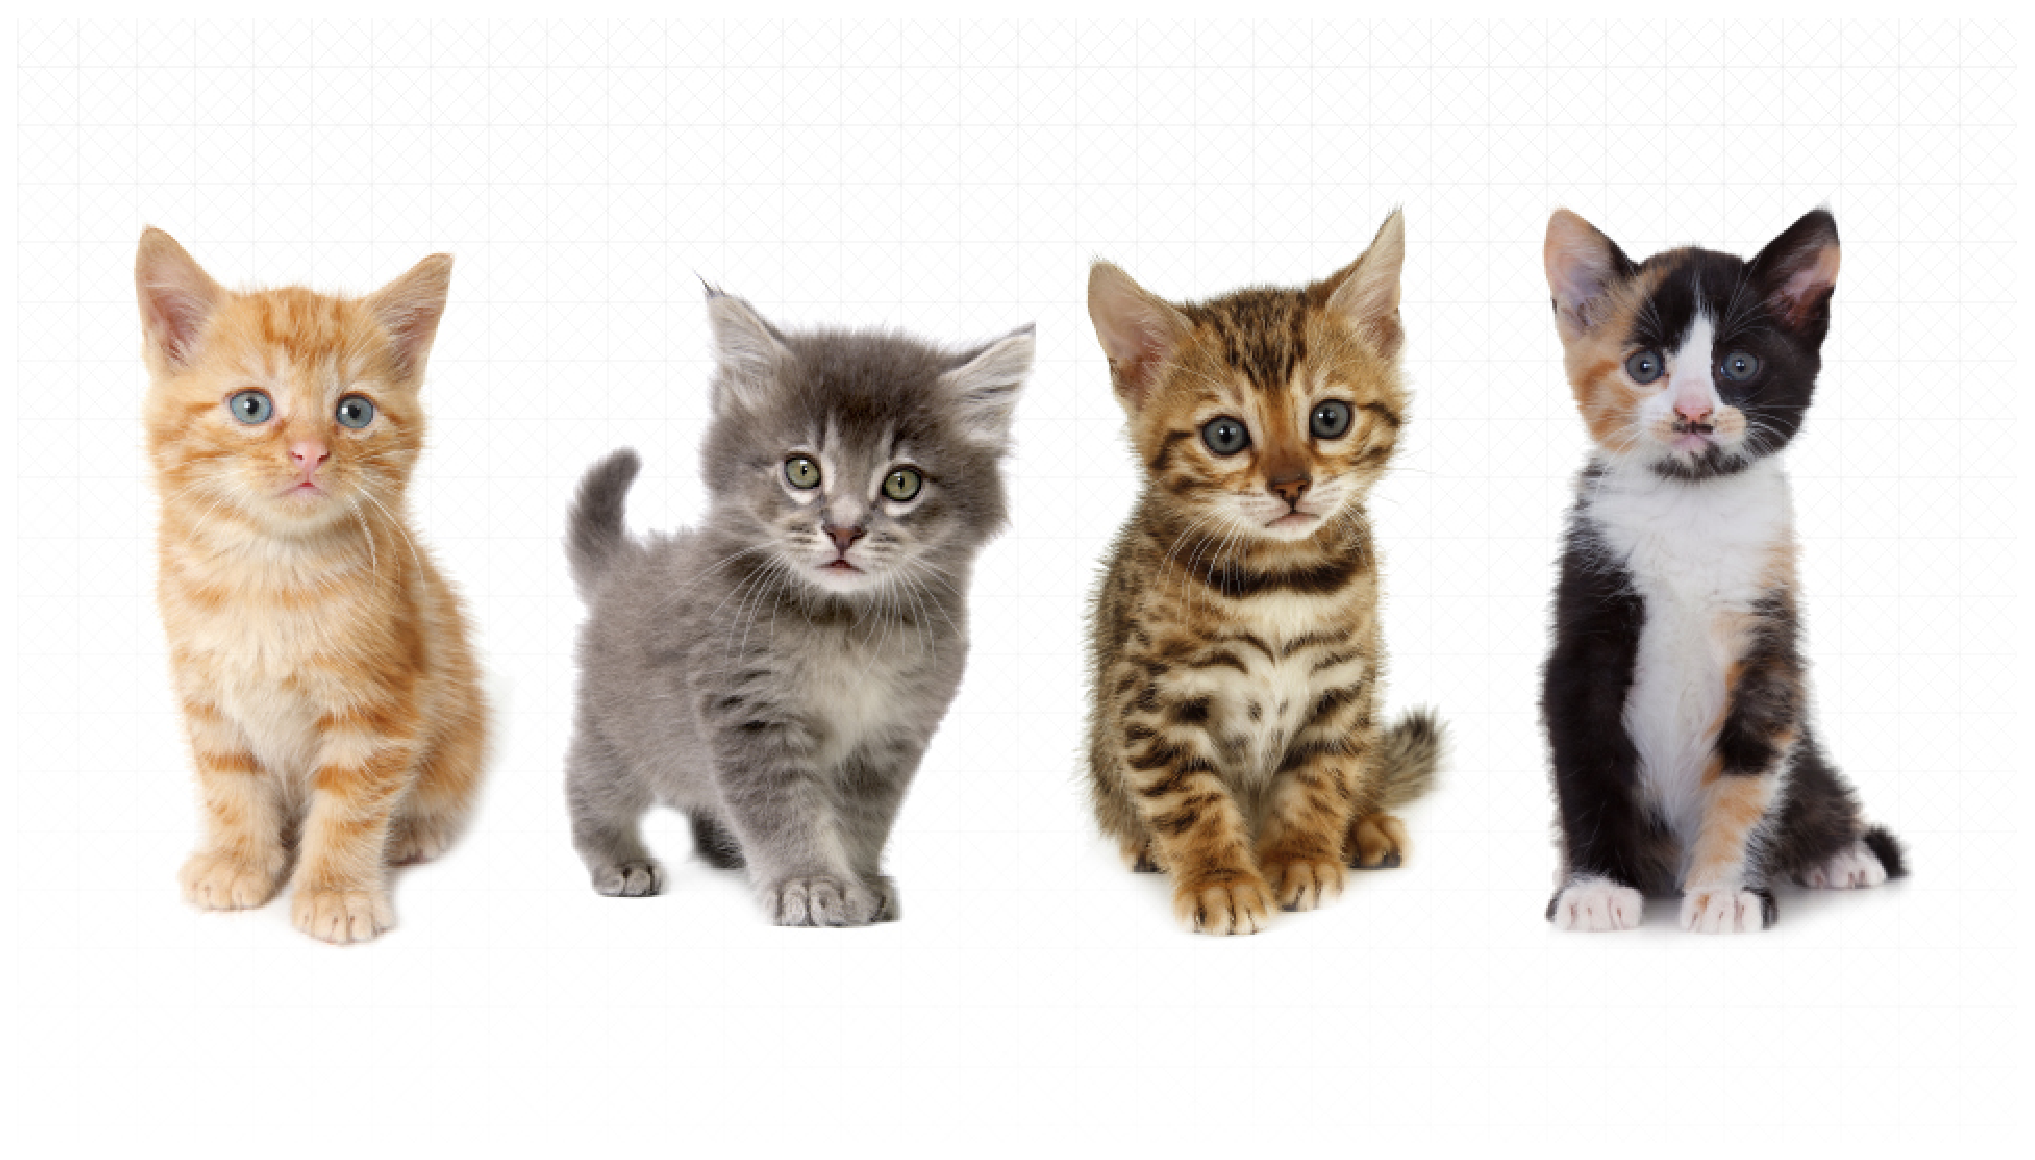
\includegraphics[width=3in]{../figures/kitty_intra_class_variation.eps}
    \end{center}
  \end{frame}

  \begin{frame}{Other Problems}
    \begin{itemize}
      \item images of the same object class are varied
      \item how to generalize to other objects?
      \item Solution: data driven approach
      \begin{itemize}
        \item provide algorithm with many varied examples of each class (i.e. 5000)
      \end{itemize}
    \end{itemize}
  \end{frame}

  \section{Neural Networks}
  \begin{frame}{What is a Neural Network?}
    \begin{itemize}
      \item collection of units (neurons) that transmit signals to one another
      \item each unit processes signal, propagates forward
      \item allows computer to learn from observational data
    \end{itemize}
    \begin{center}
      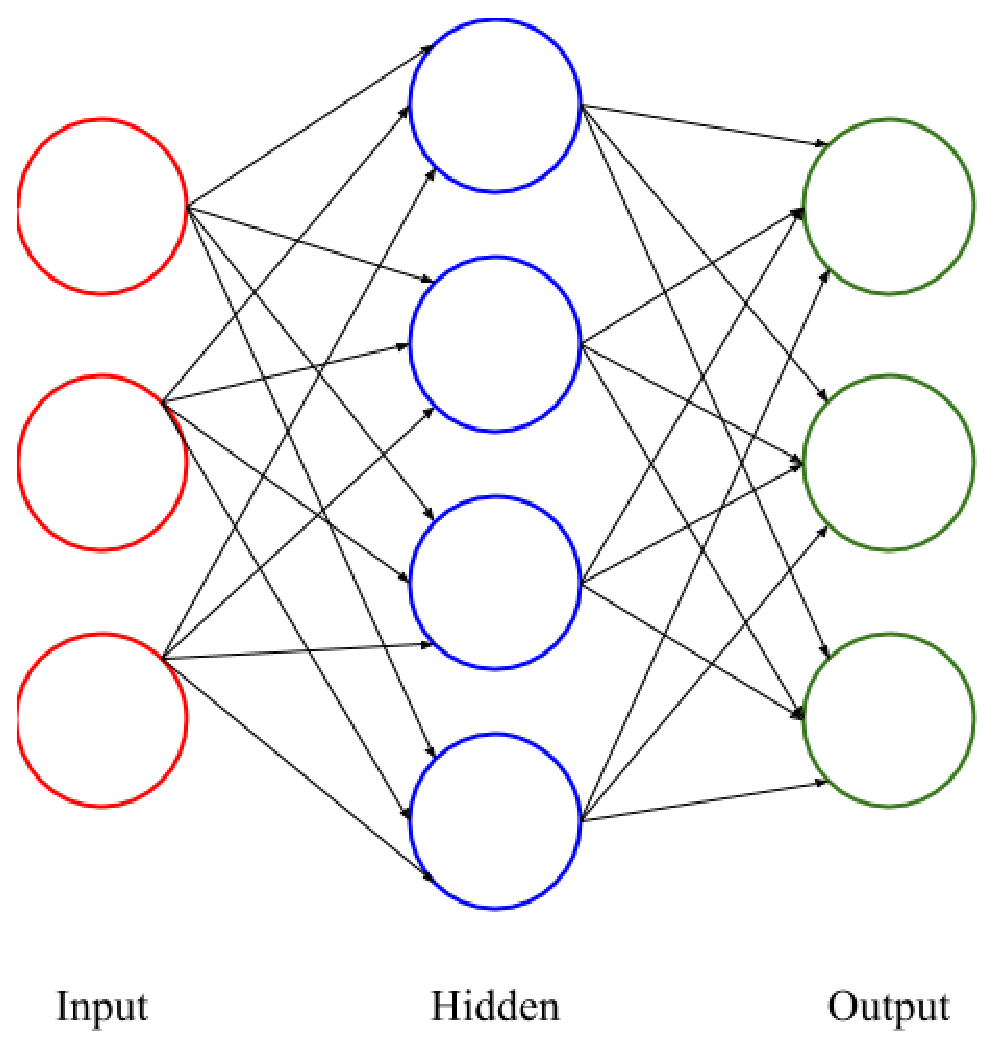
\includegraphics[height=2in]{../figures/neural_network.eps}
    \end{center}
  \end{frame}

  \section{Types of Neural Networks}
  \begin{frame}{Fully Connected Network}
    \begin{figure}[ht!]
      \centering
      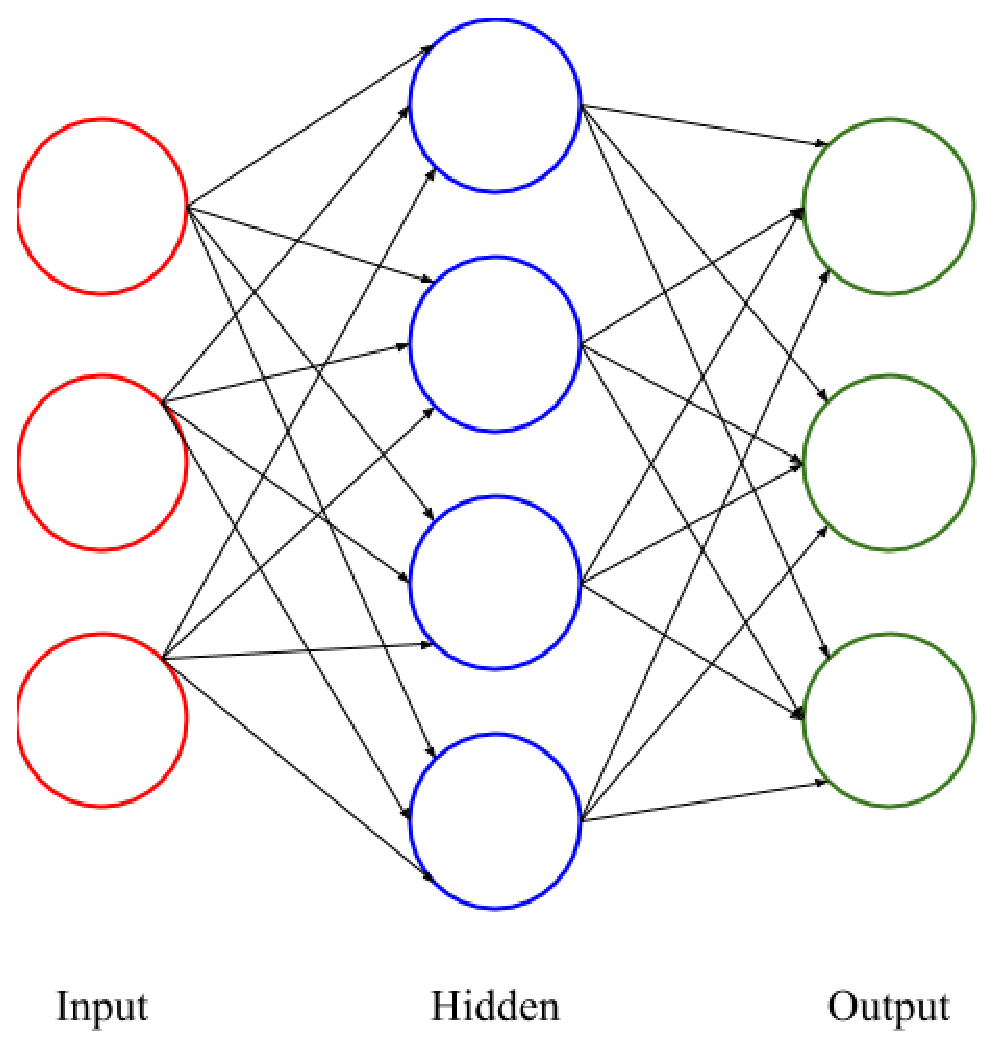
\includegraphics[height=2in]{../figures/neural_network.eps}
      \caption{Visualization of a fully-connected network.}
      \label{fig:nn}
    \end{figure} 
  \end{frame}

  \begin{frame}{Deep Neural Network}
    \begin{figure}[ht!]
      \centering
      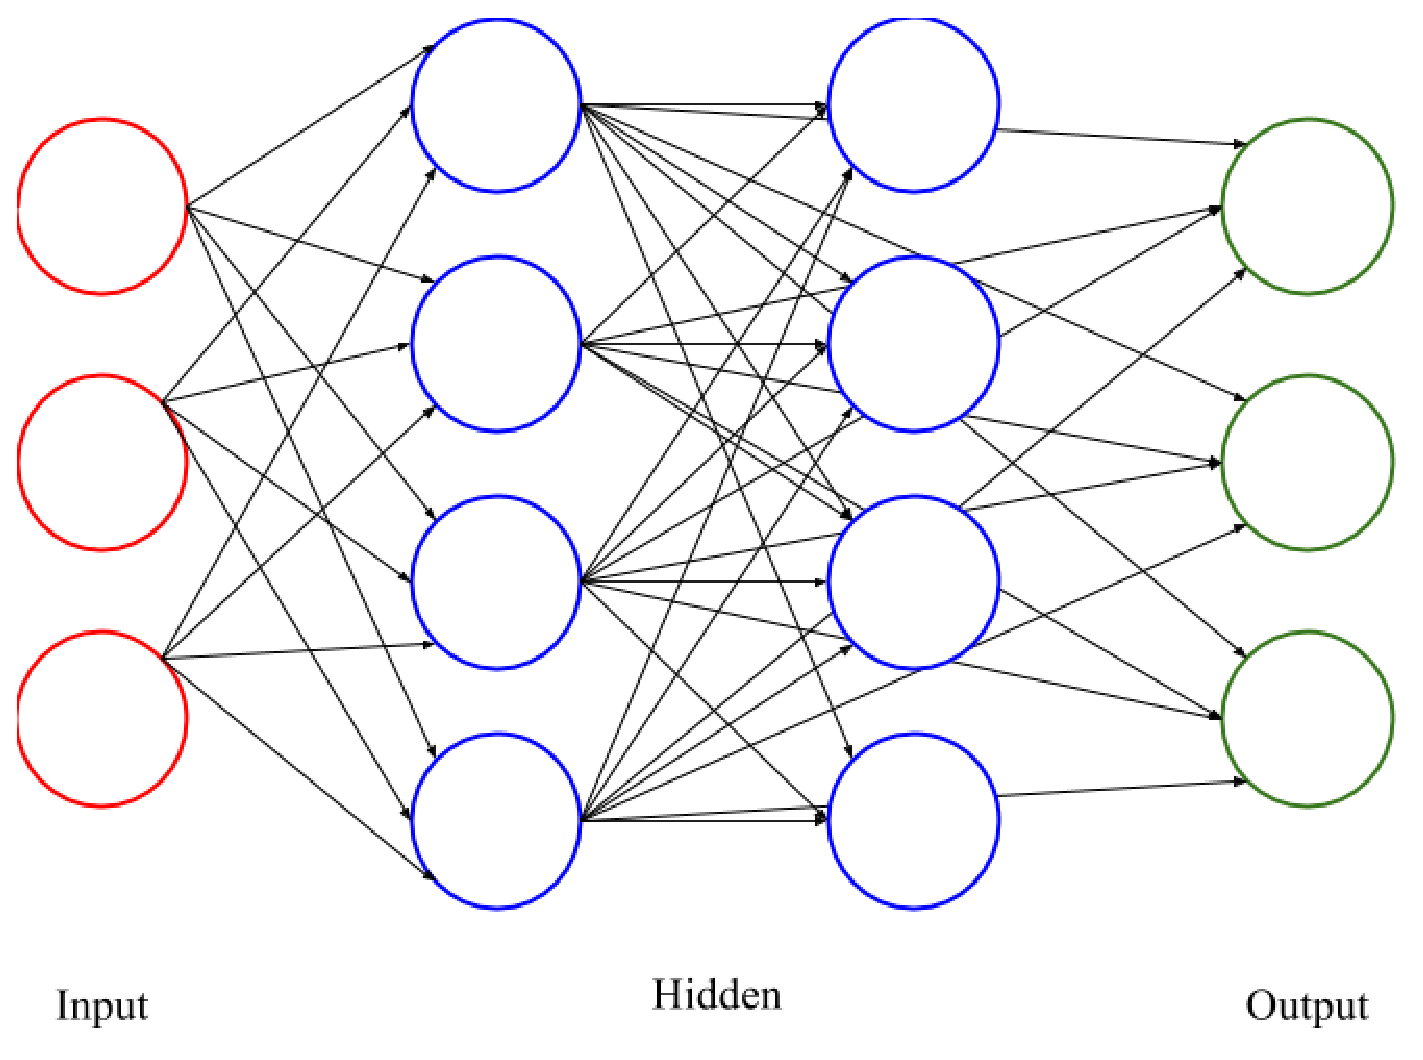
\includegraphics[height=2in]{../figures/deep_nn.eps}
      \caption{Visualization of a deep neural network}
      \label{fig:dnn}
    \end{figure}
  \end{frame}

  \begin{frame}{Convolutional Neural Network}
    \begin{figure}[ht!]
      \centering
      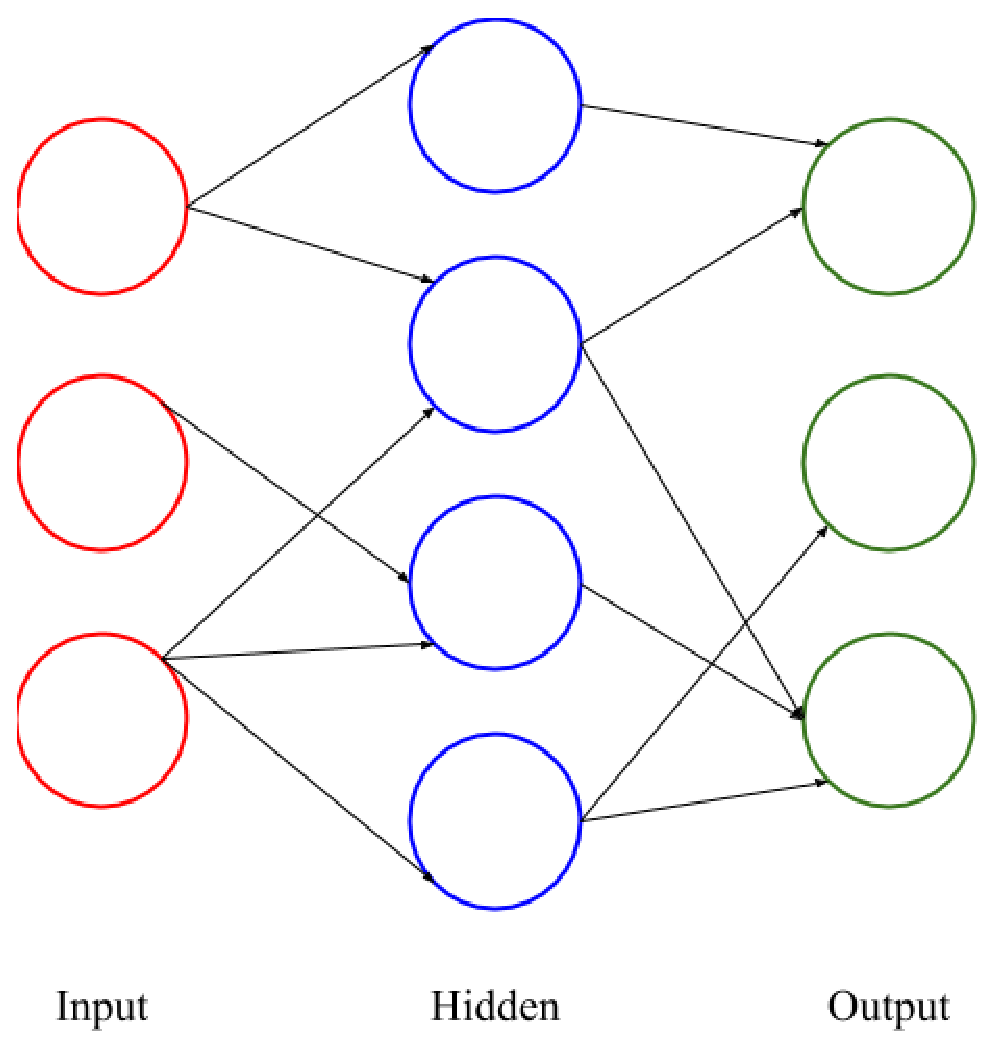
\includegraphics[height=2in]{../figures/convolutional_nn.eps}
      \caption{Visualization of a convolutional neural network}
      \label{fig:cnn}
    \end{figure}
  \end{frame}

  \begin{frame}{Datasets: MNIST}
    \begin{itemize}
      \item handwritten digit recognition
      \item $28 \times 28$ pixel, greyscale
      \item 60,000 training images, 10,000 testing images
    \end{itemize}
    \begin{center}
      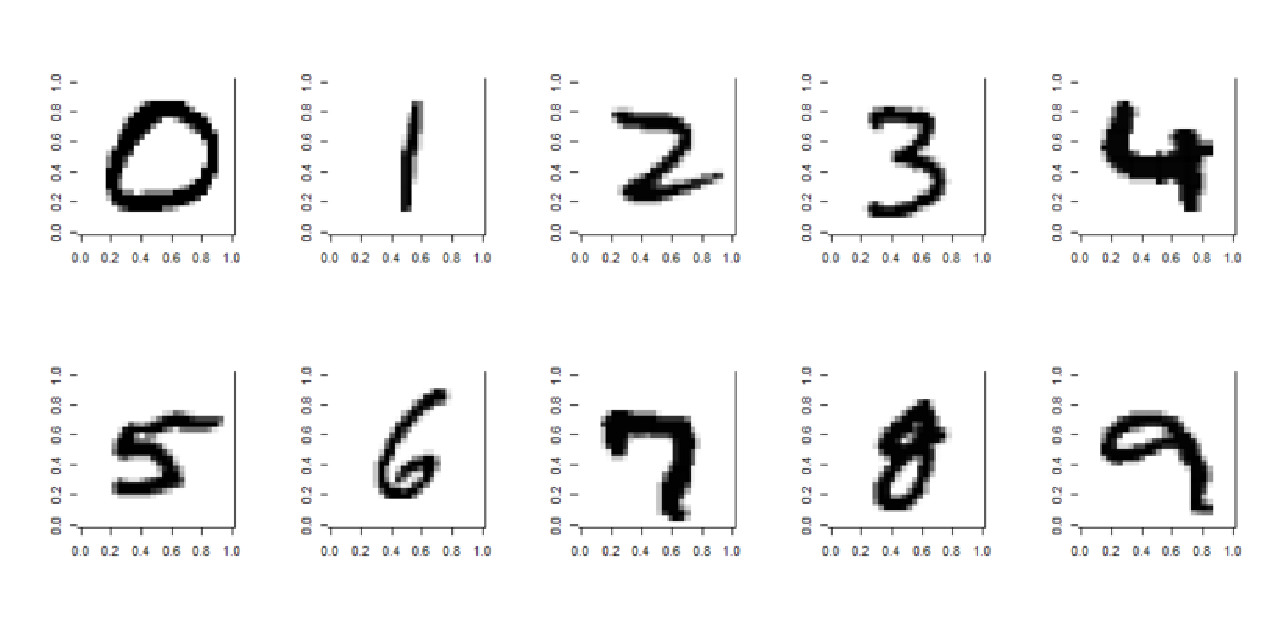
\includegraphics[height=2in]{../figures/mnist.eps}
    \end{center}
  \end{frame}

  \begin{frame}{Linear Classification}
    Essentially a 0-layer* neural network\\
    Linear classification has two important parts:
    \begin{itemize}
      \item prediction function: maps data to class scores
      \item loss function: compares predicted scores with actual labels
    \end{itemize}
  \end{frame}

  \begin{frame}{Prediction Function}
    How likely is it that each training example is part of any class?
    $$ P = XW + b $$
    \begin{itemize}
      \item $X$: training data
      \item $W$: weights
      \item $b$: bias vector
    \end{itemize}
  \end{frame}

  \begin{frame}{Loss Function}
    Evaluates $P$ based on actual data labels
    $$ L = \sum_{i=1}^m l(P_i, y_i). $$
    \begin{itemize}
      \item $y$: labels for training data
      \item $l$: loss for one training example
      \item $L$: overall loss over entire training dataset
    \end{itemize}
  \end{frame}

  \begin{frame}{Softmax Loss Function}
    $$L(P) = -\frac{1}{m} \sum_{i=1}^m \log \frac{\exp{P_{iy_i}}}
              {\sum_{j=1}^k \exp{P_{ij}}}. $$
  \end{frame}

  \begin{frame}{Gradient Descent}
    Goal: find optimal $W$ and $b$ by minimizing $L$\\
    Steps of Gradient Descent:
    \begin{enumerate}
      \item forward propogation: \begin{itemize}
        \item calculate prediction function
      \end{itemize}
      \item back propogation: \begin{itemize}
        \item calculate $\nabla P$
        \item use $\nabla P$ to calculate gradients w.r.t. model parameters
      \end{itemize}
      \item update $W$ and $b$ accordingly
    \end{enumerate}
  \end{frame}

  \section{Softmax Classifier}

  \begin{frame}{Softmax Classifier}
    Forward propagation:
    $$ P + XW + b. $$
    Back propagation:
    \begin{itemize}
      \item calculate $\nabla P$
      \item calculate $\nabla W$, $\nabla b$
    \end{itemize}
    Gradient update:
    $$ W = W - \eta \nabla W. $$
    $$ b = b - \eta \nabla b. $$
  \end{frame}

  \begin{frame}{Softmax Classifier: Deriving $\nabla P$}
    Goal: find $\frac{\partial L}{\partial W}$ and
    $\frac{\partial L}{\partial b}$ using Chain Rule.
    $$ L_i(P) = -\frac{1}{m} \left[ P_{iy_i} - \log\left( \sum_{j=1}^k \exp
    P_{ij} \right)\right] $$ for all $i$ where $1 \leq i \leq m$.

    $L_i$ depends on $P_{iv}$ $\forall$ v $1 \leq v \leq k$,
    so $\frac{\partial L_i}{\partial P_{uv}} = 0$ if $u \neq i$.

    $Y$: $m \times k$ where $Y_{ij} = 1$ if $y_i == j$, and 0 otherwise.

  \end{frame}

  \begin{frame}{Softmax Classifier: Deriving $\nabla P$}
    $$ \frac{\partial L_i}{\partial P_{iv}} = -\frac{1}{m} Y_{iv}
        + \frac{1}{m} \frac{exp(P_{iv})}{\sum_{j=1}^k \exp P_{ij}}$$.
    $$ \frac{\partial L}{\partial P_{iv}} =
       \sum_{u=1}^m \frac{\partial L_u}{\partial P_{iv}} =
       -\frac{1}{m} Y_{iv} + \frac{1}{m} \frac{exp(P_{iv})}{\sum_{j=1}^k
       \exp P_{ij}}. $$

    $$ \nabla P_{iv} = \frac{\partial L}{\partial P_{iv}} \forall i, v.$$

    $$ \nabla P = \frac{1}{m} \left[ -Y + \frac{\exp P}{\sum_{j=1}^m \exp P_j}
       \right]. $$
  \end{frame}

  \begin{frame}{Softmax Classifier: Deriving $\nabla W$}
    Facts:
    \begin{itemize}
      \item $P = XW + b$, meaning $P_{ij} = \sum_{t=1}^n X_{it}W_{tj} + b_j $
      \item $L_i$ is a function of $P_{uv}$ only if $u = i$
      \item $\nabla P_{ij} = \frac{\partial L}{\partial P_{ij}} 
            = \frac{\partial L_i}{\partial P_{ij}}$.
    \end{itemize}
  \end{frame}

  \begin{frame}{Softmax Classifier: Deriving $\nabla W$}
    \begin{align*} 
         \frac{\partial L}{\partial W_{uv}} = 
         \sum_{i=1}^m \frac{\partial L_i}{\partial W_{uv}} &= 
         \sum_{i=1}^m \sum_{j=1}^k \frac{\partial L_i}{\partial P_{i, j}}
           \frac{\partial P_{ij}}{\partial W_{uv}}\\
         &= \sum_{i=1}^m \sum_{j=1}^k
             \frac{\partial L_i}{\partial P_{ij}} X_{i, u}\\
         &= \sum_{i=1}^m \frac{\partial L_i}{\partial P_{iv}} X_{iu}\\ % confuse
         &= \sum_{i=1}^m \nabla P_{iv} X_{iu}\\
         &= \left( X^T \nabla P \right)_{uv}.
    \end{align*}

  \end{frame}

  \begin{frame}{Softmax Classifier: Deriving $\nabla W$}
    Recall: $$\frac{\partial L}{\partial W_{uv}} =  \left( X^T \nabla P
    \right)_{uv}.$$

    So:
    $$ \nabla W = X^T \nabla P. $$

    Similarly, we can show that
    $$ \nabla b = \sum_{j=0}^k P_j. $$
  \end{frame}

  \begin{frame}{Softmax Classifier: Gradient Descent Update}
    Update $W$ and $b$:
    \begin{center}
      $$ W = W - \eta \nabla W, $$
      and
      $$ b = b - \eta \nabla b, $$
      where $\eta$ is the learning rate.
    \end{center}

  \end{frame}

  \begin{frame}
  Problem:
  non-linear data?
  \end{frame}

  \section{Single Layer Neural Network}
  \begin{frame}{Single Layer}
    Steps:
    \begin{enumerate}
      \item Forward propogation:
      \begin{itemize}
        \item $ A = XW^{(1)} + b^{(1)} $
        \item $ Z = \phi(A) $
        \item $ P = ZW^{(2)} + b^{(2)} $
      \end{itemize}

      \item Backward propogation:
      \begin{itemize}
        \item calculate $\nabla W^{(1)}, \nabla W^{(2)}, \nabla b^{(1)},
              \nabla b^{(1)}, \nabla Z$
      \end{itemize}

      \item Update weights:
      \begin{itemize}
        \item e.g. $W^{(1)} = W^{(1)} - \eta \nabla W^{(1)}$
      \end{itemize}
    \end{enumerate}

    where
    $$ \phi(x) = relu(x) =
      \begin{cases}
        0 & x < 0\\
        x & x \geq 0
      \end{cases}.$$
  \end{frame}

  \begin{frame}{Single Layer}
  Fun fact: $\phi(x)$ is not differentiable at $x = 0$.\\
  Use $1(x == 0)$ instead\\
  Using Softmax Loss function as before
  \end{frame}

  \begin{frame}{Single Layer: Deriving $\nabla W^{(2)}$, $\nabla b^{(2)}$}
    Note: output layer (last layer) is identical to a Softmax Classifier, so

    $$ \nabla W^{(2)} = Z^T P, $$
    $$ \nabla b^{(2)} = \sum_{i=1}^m P_i. $$

  \end{frame}

  \begin{frame}{Single Layer: Deriving $\nabla X$, $\nabla Z$}
    \begin{align*}
      \frac{\partial L}{\partial X_{uv}} 
      =\sum_{i=1}^m \frac{\partial L_i}{X_{uv}}
      &= \sum_{i=1}^m \sum_{j=1}^k \frac{\partial L_i}{\partial P_{ij}}
          \frac{\partial P_{ij}}{\partial X_{uv}}\\
      &= \sum_{i=1}^m \sum_{j=1}^k \frac{\partial L_i}{\partial P_{ij}}
          1(i == u) W_{vj}\\
      &= \sum_{j=1}^k \sum_{i=1}^m \frac{\partial L_i}{\partial P_{ij}}
          1(i == u) W_{vj}\\
      &= \sum_{j=1}^k \frac{\partial L_u}{\partial P_{uj}} W_{vj}\\
      &= \sum_{j=1}^k \nabla P_{uj} W_{vj}
       = \left( \nabla P W^T \right) _{uv}.
    \end{align*}
  \end{frame}

    \begin{frame}{Single Layer: Deriving $\nabla X$, $\nabla Z$}
    
    Defining $\nabla X_{ij} = \frac{\partial L}{\partial X_{ij}}$, we now have
    
    $$ \nabla X = \nabla P W^T. $$
    
    % rewrite, X can be replaced with Z?
    Deriving $\nabla Z$ would be done in exactly the same way. If we define
    $\nabla Z_{uv} = \frac{\partial L}{\partial Z_{uv}}$, we now have
    
    $$ \nabla Z = \nabla P W^{(2)}. $$
      
  \end{frame}

  \begin{frame}{Single Layer: Deriving $\nabla A$}
    \begin{align*}
      \frac{\partial L}{\partial A_{uv}}
      &= \sum_{i=1}^m \frac{\partial L_i}{\partial A_{uv}}\\
      &= \sum_{i=1}^m \frac{\partial L_i}{\partial Z_{uv}} \frac{\partial
         Z_{uv}}{\partial A_{uv}}\\
      &= \frac{\partial L_u}{Z_{uv}} 1(A_{uv} > 0)\\
      &= \frac{\partial L}{Z_{uv}} 1(A_{uv} > 0)\\
      &= \nabla Z_{uv} 1(A_{uv} > 0).
    \end{align*}

    So we have
    $$ \nabla A = \nabla Z \bullet (A > 0), $$

    where $\bullet$ indicates element-wise multiplication.
  \end{frame}

  \begin{frame}{Single Layer: Deriving $\nabla W^{(1)}$, $\nabla b^{(1)}$}
    \begin{itemize}
    \item $W^{(1)}$ and $b^{(1)}$ defined similarly to $W^{(2)}$ and $W^{(2)}$
    \item have the same relationship with $A$ as $W$ and $b$ did with $P$ in
    the softmax classifier, so
    \end{itemize}
    $$ \nabla W^{(1)} = X \nabla A, $$
    $$ \nabla b^{(1)} = \sum_{i=1}^m \nabla A_i.$$

  \end{frame}

  \begin{frame}{Single Layer: Recap}
    $$ \nabla W^{(2)} = Z^T P, $$
    $$ \nabla b^{(2)} = \sum_{i=1}^m P_i, $$
    $$ \nabla X       = \nabla PW^T, $$
    $$ \nabla Z       = \nabla PW^{(2)}, $$
    $$ \nabla A       = \nabla Z \bullet (A > 0), $$
    $$ \nabla W^{(1)} = X \nabla A, $$
    $$ \nabla b^{(1)} = \sum_{i=1}^m \nabla A_i. $$
    
    for each parameter p:
      $$ p = p - \eta \nabla p. $$
  \end{frame}

  \section{Arbitrary Layer Neural Network}
  \begin{frame}{Arbitrary Layer NN}
    As before:
    \begin{enumerate}
      \item forward propagation
%      \begin{itemize}
%        \item $A^{(h)} = Z^{(h-1)}W^{(h)} + b^{(h)},$
%        \item $Z^{(h)} = \phi(A^{(h)}).$
%      \end{itemize}

      \item backward propagation
%      \begin{itemize}
%        \item calculate $\nabla A$, $\nabla W$, $\nabla b$, $\nabla Z_{out}$
%      \end{itemize}

      \item update weights
%      \begin{itemize}
%        \item e.g. $A = A - \eta \nabla A$
%      \end{itemize}
    \end{enumerate}

  \end{frame}

  \begin{frame}{Arbitrary-Layer: Forward Propagation}
    For any layer $h$ in our network:
    \begin{itemize}
      \item parameters $W^{(h)}$ and $b^{(h)}$
      \item $A^{(h)} = Z^{(h-1)} W^{(h)} + b^{(h)}$
      \item $Z^{(h)} = \phi\left( A^{(h)} \right)$
    \end{itemize}

    Notes:
    \begin{itemize}
      \item $Z^{(0)} = X$ - aka training data is input for first layer
      \item output layer: just $P = Z^{(h)} W^{(h+1)} + b^{(h+1)}$
    \end{itemize}
  \end{frame}

  \begin{frame}{Arbitrary-Layer: Back Propagation}
    For each layer $h$, calculate $\nabla Z^{(h)}$ and pass to previous layer

    $$ \nabla A = \nabla Z_{out} \bullet \left( A > 0 \right), $$
    $$ Z_{out}  = \phi\left( A \right). $$

    Just as for the single-layer network, we have
    $$ \nabla W = Z_{in} \nabla A, $$
    $$ \nabla b = \sum_{i=1}^m \nabla A_i. $$

    $$ \nabla Z_{out} = \nabla AW. $$

  \end{frame}

  \begin{frame}{Arbitrary-Layer: Update Weights}
    $$ \nabla A = \nabla Z_{out} \bullet \left( A > 0 \right), $$
    $$ \nabla W = Z_{in} \nabla A, $$
    $$ \nabla b = \sum_{i=1}^m \nabla A_i, $$
    $$ \nabla Z_{out} = \nabla AW. $$

    As before, we update our parameters with
      $$ W^{(h)} = W^{(h)} - \eta \nabla W^{(h)}, $$
      $$ b^{(h)} = b^{(h)} - \eta \nabla b^{(h)} $$
    for each layer $h$ in the network.
  \end{frame}

  \section{Implementation}

  \begin{frame}{What is oop}
    classes for robots and a room they move in
  \end{frame}

  \begin{frame}[fragile]{Softmax Classifier}

\begin{minted}{python}
class SoftmaxClassifier:
  def __init__(num_classes):
    # initialize model parameters
    ...
  def train(X, y, batch_size, num_iterations, learning_rate):
    # train classifier by calling train_batch
    ...
  def train_batch(X, y):
    # performs forward pass, back prop, gradient update
    ...
  def predict(X):
    # predict using best score for all images in X
    ...
\end{minted}

{\ttfamily SingleLayer} object will have the same structure

  \end{frame}

  \begin{frame}[fragile]{Arbitrary Layer Neural Net}
\begin{minted}{python}
class NeuralNet:
  def __init__(batch_size, epsilon, learning_rate, num_iters):
    # initialize model parameters
    ...
  def add_layer(LayerType, input_size, output_size):
    # add FullyConnected or Relu layer
    ...
  def train(X, y):
    # calls forward and backward method on batches of X
    ...
  def forward():
    # calls forward on each layer in network
    ...
  def backward():
    # calls backward on each layer in network
    ...
  def predict():
    # returns predictions using best score for all images in X
    ...
\end{minted}
  \end{frame}

  \begin{frame}[fragile]{Arbitrary Layer Neural Net}
\begin{minted}{python}
class FullyConnectedLayer:
  def __init__(master, input_size, output_size, prev=None):
    # master = NeuralNet object
    # prev = previous layer, if not first layer
    ...
  def forward():
    # preform forward pass on layer, pass to next layer
    ...
  def backward():
    # perform back propagation on layer, pass to prev layer
    ...
  
\end{minted}

also have a {\ttfamily ReluLayer} class with the same methods
  \end{frame}

  \section{Future Work}
  \begin{frame}{To Work On}
    Other Neural Network Architectures
    \begin{itemize}
      \item convolutional
    \end{itemize}
    Additional Neural Network features
    \begin{itemize}
      \item dropout % determines nodes to ignore - prevents overfitting
      \item batch normalization
    \end{itemize}
  \end{frame}

  \section{Thank-you!}
\end{document}
